% =================================================================================================================================
% The MIT Lisence:
%
% Copyright (C) 2013 Jarmo Nikkanen
%
% Permission is hereby granted, free of charge, to any person obtaining a copy of this software and associated documentation 
% files (the "Software"), to deal in the Software without restriction, including without limitation the rights to use, copy, 
% modify, merge, publish, distribute, sublicense, and/or sell copies of the Software, and to permit persons to whom the Software 
% is furnished to do so, subject to the following conditions:
%
% The above copyright notice and this permission notice shall be included in all copies or substantial portions of the Software.
%
% THE SOFTWARE IS PROVIDED "AS IS", WITHOUT WARRANTY OF ANY KIND, EXPRESS OR IMPLIED, INCLUDING BUT NOT LIMITED TO THE WARRANTIES
% OF MERCHANTABILITY, FITNESS FOR A PARTICULAR PURPOSE AND NONINFRINGEMENT. IN NO EVENT SHALL THE AUTHORS OR COPYRIGHT HOLDERS BE
% LIABLE FOR ANY CLAIM, DAMAGES OR OTHER LIABILITY, WHETHER IN AN ACTION OF CONTRACT, TORT OR OTHERWISE, ARISING FROM, OUT OF OR
% IN CONNECTION WITH THE SOFTWARE OR THE USE OR OTHER DEALINGS IN THE SOFTWARE.
% =================================================================================================================================

\documentclass[twocolumn]{report}
\usepackage{graphicx}
\newcommand{\ident}{\indent}
\newcommand{\acos}{\cos^{-1}}
\newcommand{\asin}{\sin^{-1}}
\newcommand{\atan}{\tan^{-1}}
\newcommand{\acosh}{\cosh^{-1}}
\newcommand{\asinh}{\sinh^{-1}}
\newcommand{\ve}[1]{\overrightarrow{\mathbf{#1}}}


\setlength{\hoffset}{-0.2in} \setlength{\textwidth}{17.5cm}
\setlength{\voffset}{-0.2in}\setlength{\textheight}{21cm}

\newenvironment{twocol}[0]{%
\begin{list}{}{%
\onecolumn
\setlength{\leftmargin}{0.15cm}%
\setlength{\rightmargin}{0.15cm}%
\setlength{\topmargin}{0cm}%
\setlength{\headheight}{0cm}%
\setlength{\headsep}{0cm}%
\setlength{\textheight}{24cm}%
}%
\item[]}{\end{list}}

\begin{document}

\title{
\begin{center}
\textbf{Reflections implementation}\end{center}
\begin{center}
\textbf{For}\end{center}
\begin{center}
\textbf{D3D9Client}\end{center}
\vspace{-2cm}
}

\maketitle

\begin{twocol}

\section*{Fresnel reflection}

Fresnel reflection will occur when a ray of light will hit into an "optical" material that has a refractive index $n$. Good examples of such materials are glass, water and most plastics. Fresnel reflection is highly depended from a viewing angle. In the D3D9Client we use so called Schlick's approximation of fresnel reflection. 

\begin{equation}
 R = R_0 + (1-R_0)(1-\cos\theta)^p
\end{equation}

Where the "Offset" $R_0$ is given by
\begin{equation}
R_0 = \left[\frac{1-n}{1+n}\right]^2
\end{equation}

To gain some additional properties for our function we have replaced the term $(1-R_0)$ with a multiplier $m$ resulting an equation

\begin{equation}
 R = R_0 + m(1-\cos\theta)^p
\end{equation}

Here are two plots of the equation using different values of $p$. Red curve is using value 2.0 and blue 4.0. The parameter $p$ will only effect in the view angle dependency of the fresnel reflection. The multiplier $m$ is most often set to a value $1-R_0$ and in that case the maximum reflection intensity is 1.0.

\begin{figure}[h]
	\centering
	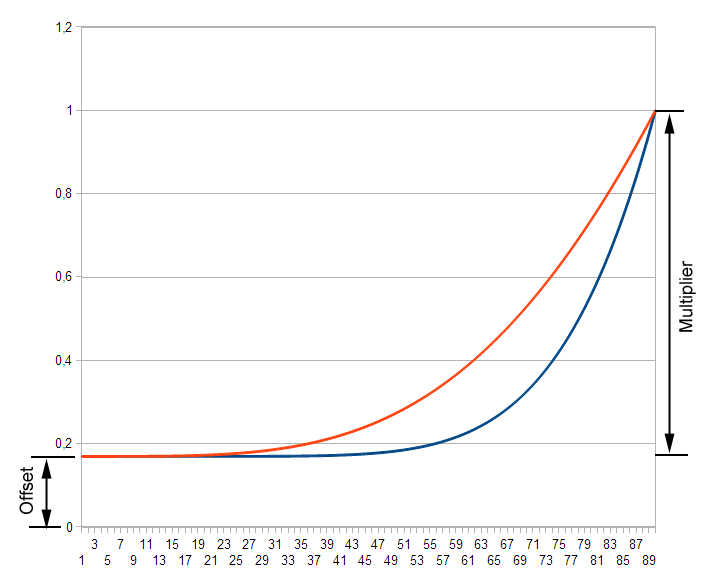
\includegraphics[width=0.6\textwidth]{images/curves.png}
	\caption{Reflection intensity as function of angle}
\end{figure}

\end{twocol}
\begin{twocol}

\section*{Reflection Model}

Here is an image about the reflection model used in D3D9Client

\begin{figure}[h]
	\centering
	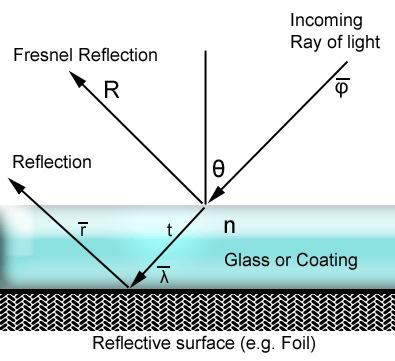
\includegraphics[width=0.35\textwidth]{images/Fresnel.png}
	\caption{Reflection model}
\end{figure}

The model consists from a fresnel reflection $R$ and a metallic reflection $r$. The lambda $\vec{\lambda}$ is a reflectivity color of the material. $t$ is a fraction of the incoming ray that is not reflected away from the interface. $\vec{\varphi}$ is the color of incoming ray of light. The value of $t$ is simply $t=1-R$.

The intensity of "metallic" reflection alone is independent from a viewing angle. However, when combined with a fresnel reflection it is given by

\begin{equation}
 \vec{r} = \vec{\lambda}t\vec{\varphi} = \vec{\lambda}(1-R)\vec{\varphi}
\end{equation}

The total reflected light is, of course, $\vec{R_{tot}}=r+R$. I suppose the fresnel reflection could take a specular color $\vec{s}$ of the material but currently it is considered to be white $\vec{s}=[1,1,1]$

\begin{equation}
\vec{R_{tot}} = (\vec{\lambda}(1-R)+\vec{s}R)\vec{\varphi}
\end{equation}

The color intensity of the diffuse surface is attennuated by the reflection intensity factor $1-|\vec{\lambda}|$. Resulting pixel color $\vec{c}$ is given by following equation where $\vec{d}$ is the color of the diffuse material or a texture.

\begin{equation}
\vec{c_{rgb}} = \vec{d_{rgb}}(1-|\vec{\lambda}|) + \vec{R_{tot}}
\end{equation}

Material/Texture alpha must be modified for alpha blending stage to make reflections visible on otherwice transparent surfaces like glass. 

\begin{equation}
\vec{c_{a}} = max(\vec{d_a}, |\vec{R_{tot}}|)
\end{equation}

In the D3D9Client we simplify the computations and we do not apply fresnel equations to incoming sunlight. A diffuse surface under a reflective coating is considered to be fully lit by the sunlight and other light sources. 

If we would take the sun angle $\sigma$ in to account then the equation would become

\begin{equation}
\vec{c_{rgb}} = \vec{d_{rgb}}(1-|\vec{\lambda}|)[1-R_0-m(1-\cos\sigma)^p] + \vec{R_{tot}}
\end{equation}

\end{twocol}
\end{document}
